\chapter{Research Description}
\label{sec:researchdesc} 

\section{Introduction}
\label{sec:introduction}

\section{Background of the Study}
\label{sec:backgroundstudy}

% What is NA Quantification and its applications ? %
Quantification of Nucleic acids (NA) is a developing research field in molecular biology for the detection and quantification expression levels of genes \cite{Huggett2015}. These NA molecules are found in deoxyribonucleic acid (DNA) and ribonucleic acid (RNA), which carries genetic information and is used as biomarkers for the detection of diseases \cite{Cao2017}. Additionally, along with the rise of bioinformatics tools, NA quantification methods are also utilized in rare mutation detection, copy number variation detection, single-cell gene and microRNA expression analysis, and next-generation sequencing \cite{Quan2018}. Outside the scope of molecular biology, its application has also found its way in forensic research \cite{Whale2013}, medical diagnosis, environmental monitoring, and food safety analysis \cite{Cao2017}.


% How to Quantify NA Quantification with (dPRC) ? %
To be able to determine the concentration of target NAs, NA detection is naturally a pre-requisite. There are, however, NAs of interests that have very low concentrations to the point that it becomes undetectable in existing detection technologies. This problem is solved by amplifying the NA sequences using Polymerase Chain Reaction (PCR), a widely-used method for NA amplification since its invention in the 1980s \cite{Cao2017}. PCR can multiply specific NA sequences in DNA or RNA from low concentrations to millions of copies. This method exposes the NA sequences mixed with chemical components in a series of 20 to 40 temperature cycles. In each cycle, PCR doubles the NA molecule; theoretically producing \(2^n\) molecules after \(n\) cycles \cite{Quan2018}.

After PCR amplification, absolute NA quantification is achieved using digital Polymerase Chain Reaction (dPCR) technique. This equally divides the NA samples into thousands of partitions; each of these partitions is evaluated as either off or on, or in this context, labeled as positive or negative, hence the term "digital" \cite{Cao2017}.

The dPCR workflow, as illustrated in \figref{fig:dpcrWorkflow}, is typically a sequential procedure of extracting the sample from an organism, preparing the sample, distribution of the sample to partitions, PCR amplification and detection, and finally is estimated using a Poisson correction factor. In \cite{Jacobs2014}, it was emphasized that every step of the dPCR workflow inevitably allows for the introduction of different sources of variation. These variance components within the dPCR workflow is shown in \figref{fig:workflowVariation}. 

\begin{figure}[h]
    \centering
    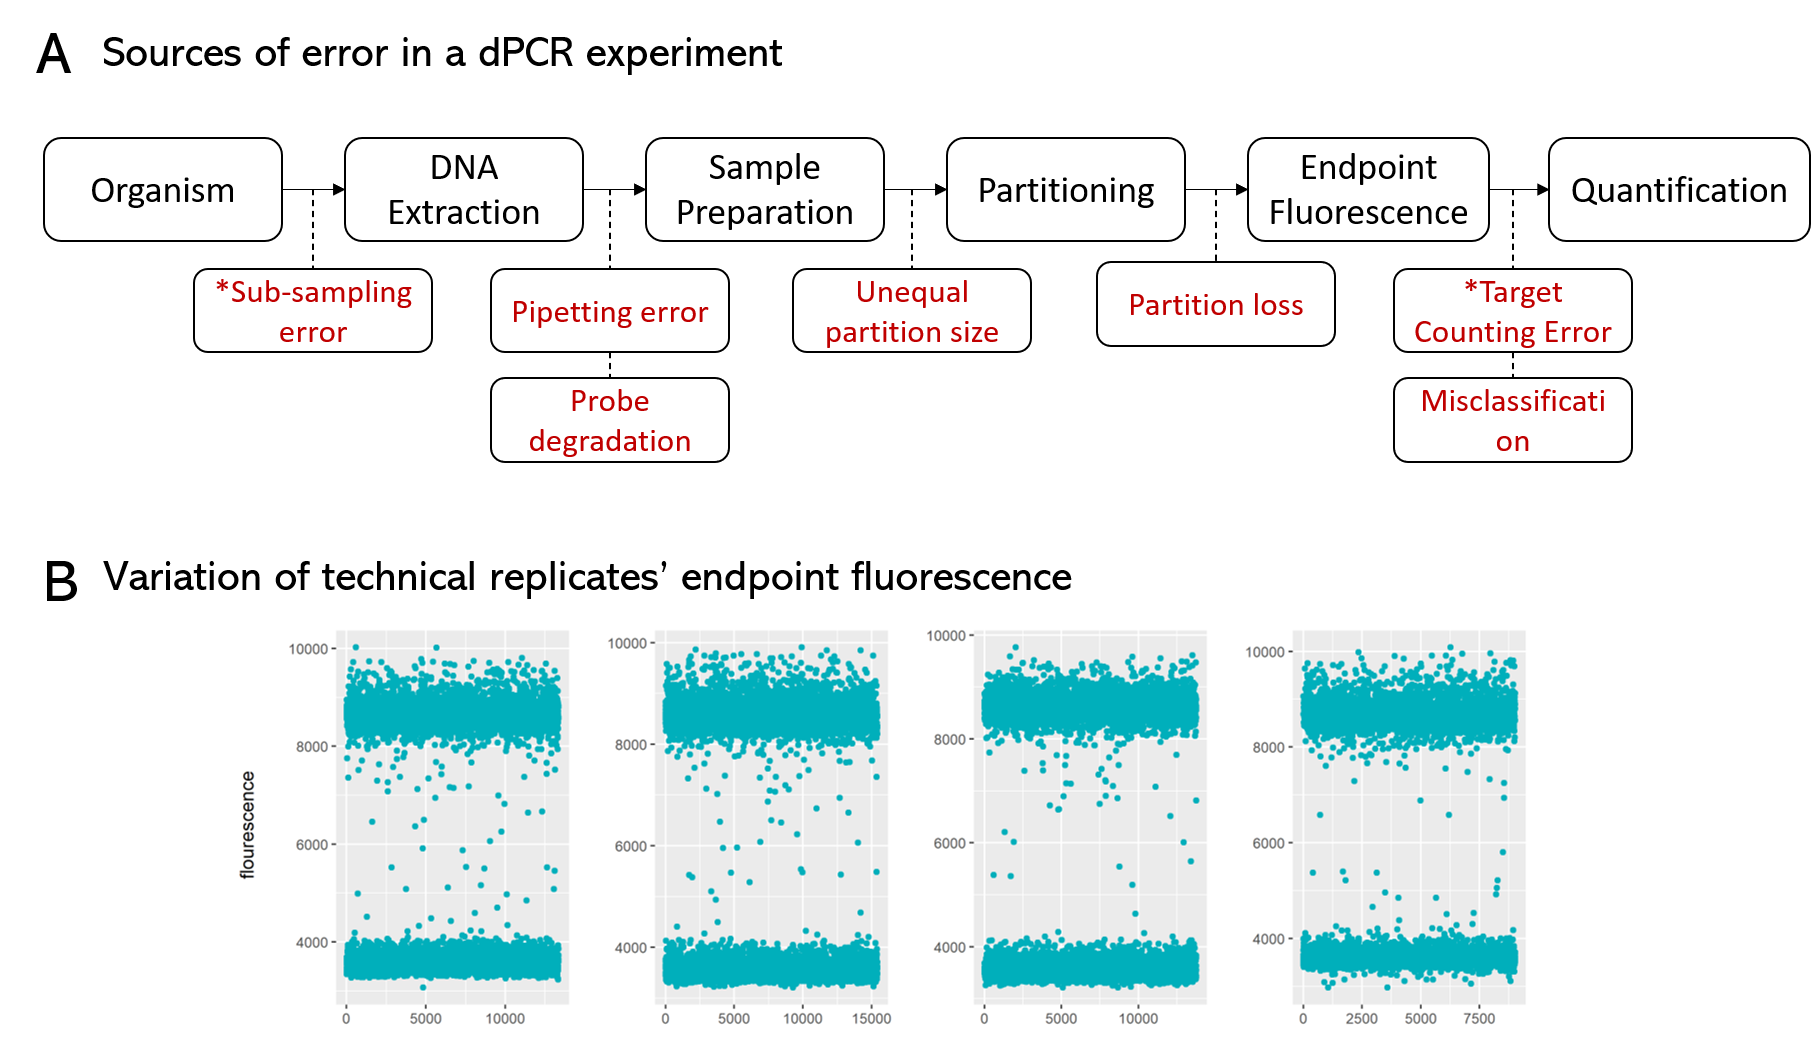
\includegraphics[max size={\textwidth}{\textheight}]{dpcrWorkflow.png}
    \caption{The dPCR workflow}
        \label{fig:dpcrWorkflow}
\end{figure}

\begin{figure}[h]
    \centering
    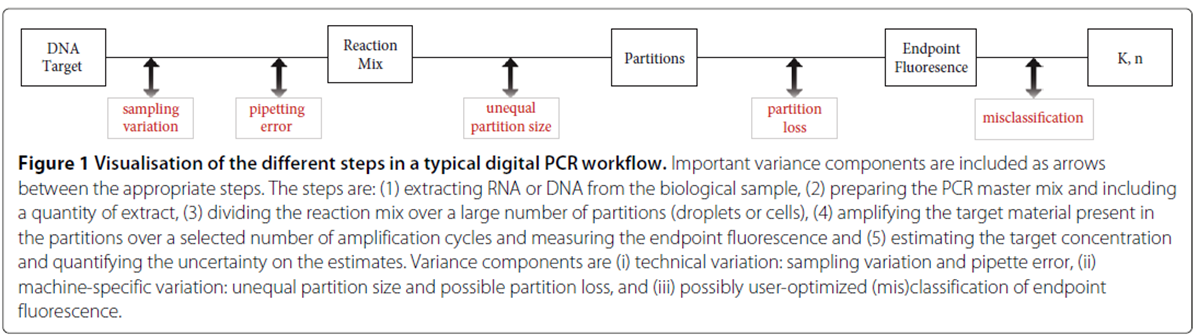
\includegraphics[max size={\textwidth}{\textheight}]{workflowVariation.png}
    \caption{Potential variation components between steps of the dPCR workflow}
        \label{fig:workflowVariation}
\end{figure}

When 


\section{Statement of the Problem}
\label{sec:statementprob}

\section{Significance of the Study}
\label{sec:significancestudy}

\section{Scope and Limitations}
\label{sec:significance}
